\chapter{Arsitektur dalam Rancangan Implementasi}
\label{appendix:architecture}

\begin{figure}[ht]
    \centering
    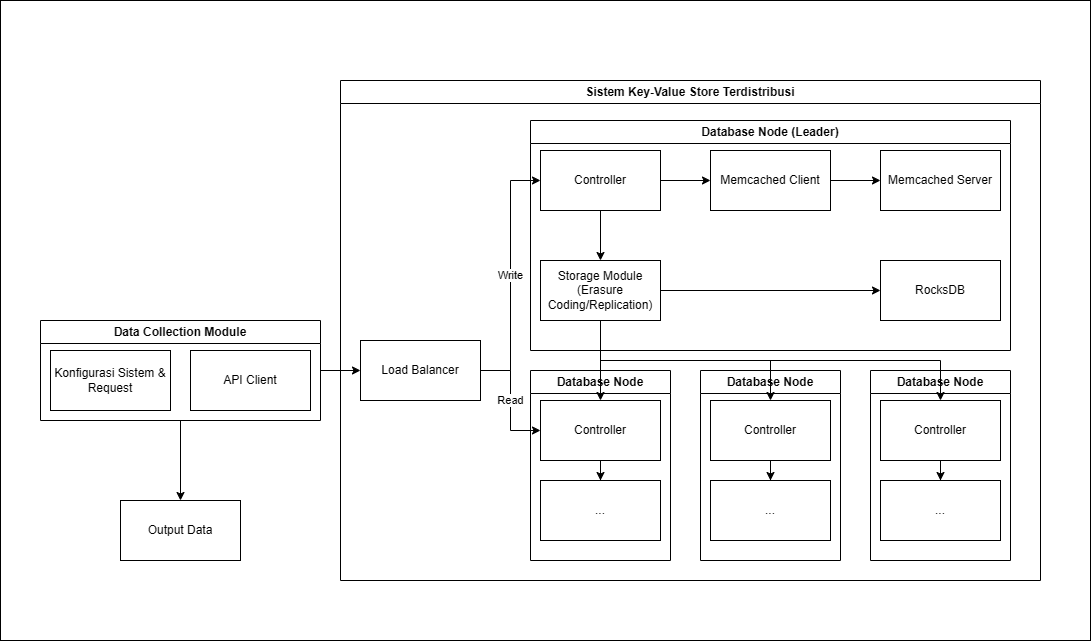
\includegraphics[width=0.95\textwidth]{resources/appendix/general-architecture.png}
    \caption{Gambaran Umum Arsitektur Sistem Eksperimen}
    \label{fig:general-architecture}
\end{figure}

Arsitektur dari sistem mengasumsikan kebutuhan untuk konsistensi yang tinggi. Untuk mencapai konsistensi tersebut, operasi \textit{write} dilakukan secara \textit{synchronous} dengan distribusi replikasi dan \textit{erasure coding} dianggap selesai ketika nilai ketahanan yang diinginkan sudah tercapai. Sistem terdistribusi akan mengadopsi pola \textit{leader-follower} untuk memudahkan sinkronisasi data. Pemilihan \textit{leader} dan pemastian transaksi akan dilakukan menggunakan algoritma konsensus \textit{paxos} yang disesuaikan dengan kebutuhan. Diagram gambaran umum arsitektur sistem dapat dilihat pada gambar \ref{fig:general-architecture}.

Operasi akan disalurkan melalui sebuah \textit{load-balancer} sebelum mencapai \textit{database node}. Operasi \textit{write} akan secara ekslusif disalurkan pada \textit{leader}. Kemudian untuk ketahanan, data akan didistribusikan pada \textit{follower} sesuai dengan konfigurasi modul \textit{redundancy}. Sementara itu, operasi \textit{read} dapat dilakukan pada \textit{database node} manapun. Pada sistem \textit{erasure coding}, jika pada \textit{node} tersebut tidak terdapat nilai data yang dicari, maka \textit{node} akan melakukan \textit{request} ke semua node lainnya untuk melakukan rekonstruksi data. Penjelasan lebih lanjut terkait \textit{flow} operasi akan dijelaskan pada lampiran \ref{appendix:flow}.
